\documentclass[twocolumn,final]{article}

\usepackage{amsmath}
\usepackage{amsfonts}
\usepackage{graphicx}
\usepackage{booktabs}
\usepackage{url}
\usepackage{color}

\title{Classifying brain states induced by comlex visual stimuli}

\author{Andrew Floren\\
1 University Station, C0803\\
The University of Texas at Austin\\
Austin TX, 78712-1084 USA\\
afloren@mail.utexas.edu\\
(214) 384-2895\\}

\date{}

\bibliographystyle{acm}

\begin{document}

\maketitle

\begin{abstract}
abstract
\end{abstract}

\tableofcontents

\section{Introduction}
In traditional fMRI experiments, investigators seek to identify relationships between the measured BOLD signal and a carefully designed stimulus in order to tease out the purpose of particular brain regions.
Recently, a new trend has developed where researchers are instead looking to predict what stimulus was presented given the measured BOLD signal \cite{Haxby2001,Mitchell2003,Haynes2006}.
While successful, most of these experiments involve presenting static images from a limited number classes such as faces and places.
Then, the researchers try to classify which image or class of images was presented during each frame by analyzing the measured BOLD signal using machine learning classifiers.
While this has proven to be a successful approach, it does not mimic the dynamic environment in which brains have evolved.
Our goal is to analyze brain function with dynamically changing stimuli that portray real world experiences.
Further, we were interested to see what information could be gleaned from the BOLD signal beyond object categories.
We used virutal world technology to specify the stimuli in detail.
Given our long-term interest in PTSD, we created a virtual town intended to suggest the kinds of real-world settings currently encountered by our military forces.
Virtual character representing firnedly forces and hostile combatentswere presented in a virtual town.
We then trained linear SVMs (support vector machines) and feed forward neural networks to predict the number of characters in each stimulation.

\section{Methods}

\subsection{Stimulus}
We developed a virtual reality environment similar to many popular first person video games using the Unreal Engine 2 SDK \cite{UnrealEngine2}.
The stimuli is dynamically rendered and presented from the point of view of a camera moving through this virutal environmentw hile characters are presented.
The stimulus employs a classic block design, in which the viewpoint moves for 15 seconds through the virtual environment (an example frame is presented in figure \ref{fig:stimulus-movement}), then pauses for 15 seconds during which a group of characteres fades into view (an example frame is presented in figure \ref{fig:stimulus-characters}).
The camera is constantly moving (even during the character presention periods the camera slowly pans and rotates) and the characters are animated so that the presented scene is never static.
The number of characters varies from one to six as well as the locaiton of eah character in each presentation in a quasi-random fashion.
Specifically, a presentation with a particular number of characters appears twice in each run, however the order of these presentations was randomized.
It should be noted that, this random ordering was generated once and held constant between subjects.
Additionally, even between character presentations with the same number of characters, the locations of those characters varies considerably as seen in figure \ref{fig:stimulus-location}.
Each run consists of 12 alternations between moving through the virtual environment and character presentations. 
In each scanning session, 4 to 6 runs were collected.

\begin{figure}[!htbp]
\centering
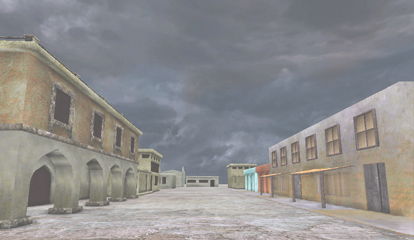
\includegraphics[width=0.5\textwidth]{figures/stimulus-movement}
\caption{An example frame from the stimulus while the camera is moving through the virtual envronment.}
\label{fig:stimulus-movement}
\end{figure}

\begin{figure}[!htbp]
\centering
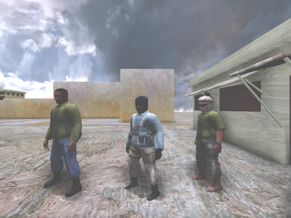
\includegraphics[width=0.5\textwidth]{figures/stimulus-characters}
\caption{An example frame from the stimulus while characters are being presented.}
\label{fig:stimulus-characters}
\end{figure}

\begin{figure}[!htbp]
\centering
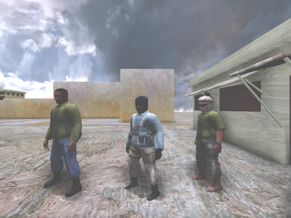
\includegraphics[width=0.5\textwidth]{figures/stimulus-location}
\caption{Two example frames depicting character presentations with two characters. The locations of the two characters varies considerably between the two frames.}
\label{fig:stimulus-location}
\end{figure}

\subsection{fMRI}
We collected whole brain scans using a GRAPPA-accelerated EPI, with a 2.5 second TR and 2.5 mm cubic voxels on 40 slices that covered the majority of each subjects brain (see figure \ref{fig:rx}).

\begin{figure}[!htbp]
\centering
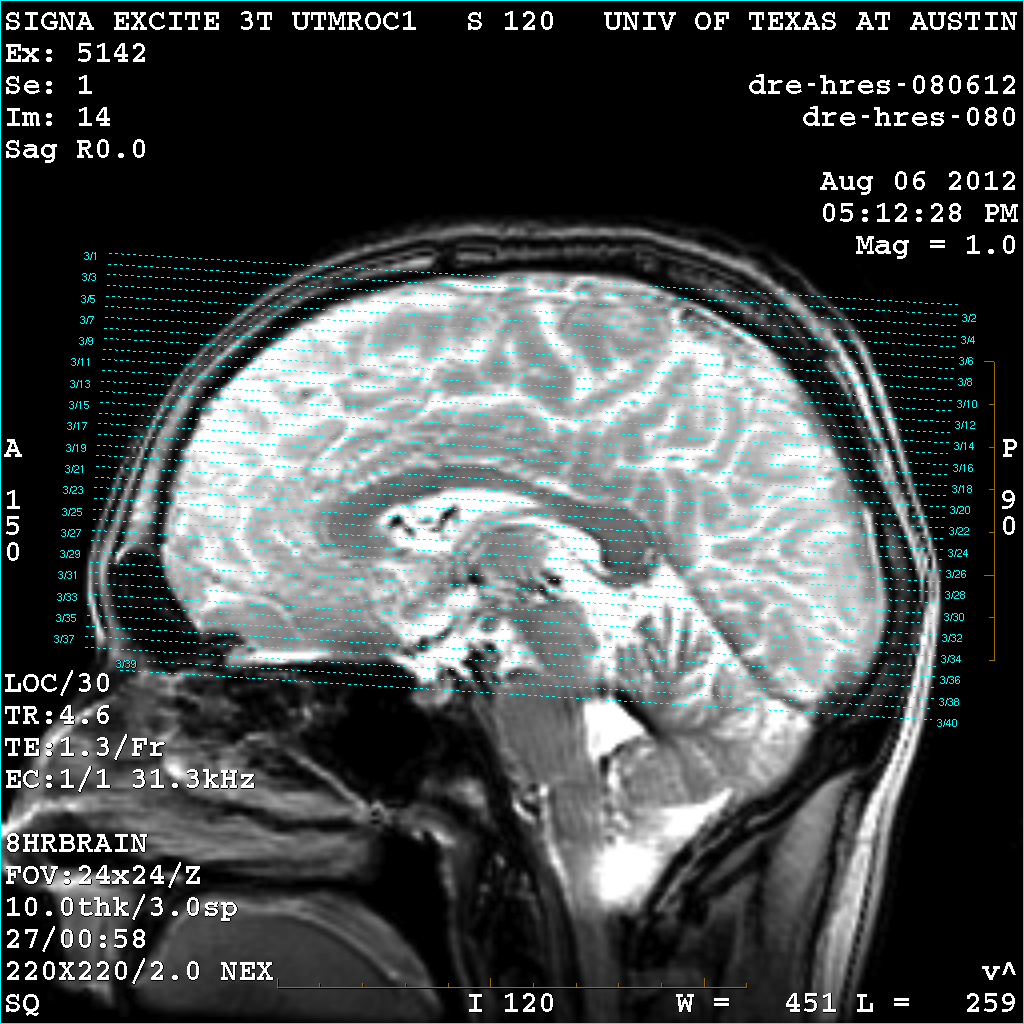
\includegraphics[width=0.5\textwidth]{figures/rx}
\caption{An example prescription from one of the subjects.}
\label{fig:rx}
\end{figure}

\subsection{Preprocessing}
We performed motion compensation and slice timing corrections. 
Additionally, we applied a Wiener filter deconvolution using a generic difference-of-gamma HRF \cite{Boynton1996} to shift the peak response in time so that it is aligned with the stimulus that caused it.
Given a system:
\begin{equation}
y(t) = h(t) \ast x(t) + n(t)
\end{equation}
Want to find $g(t)$ such that 
\begin{equation}
\hat{x}(t) = g(t) \ast y(t)
\end{equation}
minimizes
\begin{equation}
\sum_{t}{\left( \hat{x}(t) - x(t) \right)^{2}}
\end{equation}
The solution is most easily expressed in the Fourier domain where the solution is:
\begin{equation}
g(t) \xrightarrow{\mathcal{F}} \frac{H^{*}(f)}{\left|H(f)^{2}\right| + \mbox{SNR}^{-1}(f)}
\end{equation}

Finally, we reduce the dimensionality of the problem by masking out a subset of he volume using a harmonic power analysis.
We selected N ($\sim$3000) voxels with the greatest power at the frquency of the block alternation and its harmonics.
In other words, we selected the vosels that responded in any fashion that covaried with the stimulus alternations.
Thus, the selection was based only on the alternation between presentation of characters and the empty town, without regard to the number of characters.
Let $y(t)$ be the recorded discrete time series at some voxel.
Then let $Y(f)$ be the discrete Fourier transform of $y(t)$.
The harmonic power of that time series is defined as:
\begin{equation}
\frac{\sum_{i = 1}^{M}{\left|Y(i \cdot N)\right|^{2}}}{\sum_{f}{\left|Y(f)\right|^{2}}}
\end{equation}
Where $M$ is the number of harmonics and $N$ is the frequency of interest, in our case the period of the block alternations.
\subsection{Classification}
Using the timer series of data from these voxels, we trained a linear SVM and a feed forward neural network.
Thes algorithms were trained and validated using a cross-fold approach \cite{Kohavi1995}.
Each frame or point in the time series was treated as a separate data point instead of averaging across the block.
However, data points from the same block were not allowed to be split across the training and test set in order to avoid issues with noise correlations causing overly optimistic performace estimates.
This data splitting strategy is depictied in figure \ref{fig:data-split}.

The performance of each classifer was characterized by its micro-averaged $F$-measure. 
The $F$-measure for a single class is described by the following equations:
\begin{equation}
\mbox{precision} = \frac{tp}{tp + fp}
\label{eqn:precision}
\end{equation}
\begin{equation}
\mbox{recall} = \frac{tp}{tp + fn}
\label{eqn:recall}
\end{equation}
\begin{equation}
F = 2 \cdot \frac{\mbox{precision} \cdot \mbox{recall}}{\mbox{precision} + \mbox{recall}}
\label{eqn:f1}
\end{equation}
Where $tp$ is the number of true positives, $fp$ is the number of false positives, and $fn$ is the number of false negatives.
The $F$-measure is a more robust measure of the performance of a classifier than either precision or recall alone.
For example, if the classifier labeled everything as positive then the recall would be perfect but the precision would be at chance levels.
On the other hand, if the classifier only labeled examples it was highly confidant in as positive then precision would be high but recall would be low.
The $F$-measure can be generalized for multiple classes by summing true positive, false positive, and false negative counts across all classes.
\begin{equation}
\mbox{precision}_{avg} =\frac{\sum_{i}^{M}{tp_{i}}}{\sum_{i}^{M}{\left( tp_{i} + fp_{i} \right)}}
\end{equation}
\begin{equation}
\mbox{recall}_{avg} = \frac{\sum_{i}^{M}{tp_{i}}}{\sum_{i}^{M}{\left( tp_{i} + fn_{i} \right)}}
\end{equation}
Where $M$ is the number of classes.
The multi-class $F$-measure is then calculated as:
\begin{equation}
F_{avg} = 2 \cdot \frac{\mbox{precision}_{avg} \cdot \mbox{recall}_{avg}}{\mbox{precision}_{avg} + \mbox{recall}_{avg}}
\end{equation}
This is known in the literature as the  micro-averaged $F$-measure.

\begin{figure}[!htbp]
\centering

\includegraphics[width=0.5\textwidth]{figures/placeholder}
\caption{The strategy employed for splitting up the train, test, and validate sets to minimize optimistic performance estimates.}
\label{fig:data-split}
\end{figure}

\subsection{Sensitivity Analysis}
Sensitivity analysis \cite{Zurada1994}:
\begin{equation}
Sensitivity analysis
\end{equation}

\section{Results}

\begin{table}[!htbp]
\centering
\begin{tabular}{l *{10}{c}}
\toprule
& \multicolumn{2}{c}{Frame} & \multicolumn{2}{c}{Block} & \multicolumn{2}{c}{Half-Run} & \multicolumn{2}{c}{Run} & \multicolumn{2}{c}{Session} \\
\cmidrule(lr){2-3} \cmidrule(rl){4-5} \cmidrule(rl){6-7} \cmidrule(rl){8-9} \cmidrule(l){10-11}
Subject	& SVM & NN & SVM & NN & SVM & NN & SVM & NN & SVM & NN \\
\midrule
A		& 0.6 & 0.6 & 0.6 & 0.6 & 0.6 & 0.6 & 0.6 & 0.6 & 0.6 & 0.6 \\
B		& 0.6 & 0.6 & 0.6 & 0.6 & 0.6 & 0.6 & 0.6 & 0.6 & 0.6 & 0.6 \\
C		& 0.6 & 0.6 & 0.6 & 0.6 & 0.6 & 0.6 & 0.6 & 0.6 & 0.6 & 0.6 \\
D		& 0.6 & 0.6 & 0.6 & 0.6 & 0.6 & 0.6 & 0.6 & 0.6 & 0.6 & 0.6 \\
E		& 0.6 & 0.6 & 0.6 & 0.6 & 0.6 & 0.6 & 0.6 & 0.6 & 0.6 & 0.6 \\
Average	& 0.6 & 0.6 & 0.6 & 0.6 & 0.6 & 0.6 & 0.6 & 0.6 & 0.6 & 0.6 \\
\bottomrule 
\end{tabular}

\caption{
The multi-class $F_1$ scores of the linear SVM and the feed forward neural network after a 10 fold cross-validation for all 5 subjects. 
Every frame was shuffled independently into the train, test, and validation sets.}
\label{tab:frame-shuffle}
\end{table}

\begin{table}[!htbp]
\centering
\begin{tabular}{l *{10}{c}}
\toprule
& \multicolumn{2}{c}{Frame} & \multicolumn{2}{c}{Block} & \multicolumn{2}{c}{Half-Run} & \multicolumn{2}{c}{Run} & \multicolumn{2}{c}{Session} \\
\cmidrule(lr){2-3} \cmidrule(rl){4-5} \cmidrule(rl){6-7} \cmidrule(rl){8-9} \cmidrule(l){10-11}
Subject	& SVM & NN & SVM & NN & SVM & NN & SVM & NN & SVM & NN \\
\midrule
A		& 0.6 & 0.6 & 0.6 & 0.6 & 0.6 & 0.6 & 0.6 & 0.6 & 0.6 & 0.6 \\
B		& 0.6 & 0.6 & 0.6 & 0.6 & 0.6 & 0.6 & 0.6 & 0.6 & 0.6 & 0.6 \\
C		& 0.6 & 0.6 & 0.6 & 0.6 & 0.6 & 0.6 & 0.6 & 0.6 & 0.6 & 0.6 \\
D		& 0.6 & 0.6 & 0.6 & 0.6 & 0.6 & 0.6 & 0.6 & 0.6 & 0.6 & 0.6 \\
E		& 0.6 & 0.6 & 0.6 & 0.6 & 0.6 & 0.6 & 0.6 & 0.6 & 0.6 & 0.6 \\
Average	& 0.6 & 0.6 & 0.6 & 0.6 & 0.6 & 0.6 & 0.6 & 0.6 & 0.6 & 0.6 \\
\bottomrule 
\end{tabular}

\caption{
The multi-class $F_1$ scores of the linear SVM and the feed forward neural network after a 10 fold cross-validation for all 5 subjects. 
Every block was shuffled independently into the train, test, and vaidation sets.}
\label{tab:block-shuffle}
\end{table}

\begin{table}[!htbp]
\centering
\begin{tabular}{l *{10}{c}}
\toprule
& \multicolumn{2}{c}{Frame} & \multicolumn{2}{c}{Block} & \multicolumn{2}{c}{Half-Run} & \multicolumn{2}{c}{Run} & \multicolumn{2}{c}{Session} \\
\cmidrule(lr){2-3} \cmidrule(rl){4-5} \cmidrule(rl){6-7} \cmidrule(rl){8-9} \cmidrule(l){10-11}
Subject	& SVM & NN & SVM & NN & SVM & NN & SVM & NN & SVM & NN \\
\midrule
A		& 0.6 & 0.6 & 0.6 & 0.6 & 0.6 & 0.6 & 0.6 & 0.6 & 0.6 & 0.6 \\
B		& 0.6 & 0.6 & 0.6 & 0.6 & 0.6 & 0.6 & 0.6 & 0.6 & 0.6 & 0.6 \\
C		& 0.6 & 0.6 & 0.6 & 0.6 & 0.6 & 0.6 & 0.6 & 0.6 & 0.6 & 0.6 \\
D		& 0.6 & 0.6 & 0.6 & 0.6 & 0.6 & 0.6 & 0.6 & 0.6 & 0.6 & 0.6 \\
E		& 0.6 & 0.6 & 0.6 & 0.6 & 0.6 & 0.6 & 0.6 & 0.6 & 0.6 & 0.6 \\
Average	& 0.6 & 0.6 & 0.6 & 0.6 & 0.6 & 0.6 & 0.6 & 0.6 & 0.6 & 0.6 \\
\bottomrule 
\end{tabular}

\caption{
The multi-class $F_1$ scores of the linear SVM and the feed forward neural network after an 8 fold cross-validation for all 5 subjects. 
Every epoch was shuffled independently into the train, test, and vaidation sets. 
Only 8 folds were used because most subjects have only 8 epochs of data collected.}
\label{tab:epoch-shuffle}
\end{table}

\begin{table}[!htbp]
\centering
\begin{tabular}{l *{10}{c}}
\toprule
& \multicolumn{2}{c}{Frame} & \multicolumn{2}{c}{Block} & \multicolumn{2}{c}{Half-Run} & \multicolumn{2}{c}{Run} & \multicolumn{2}{c}{Session} \\
\cmidrule(lr){2-3} \cmidrule(rl){4-5} \cmidrule(rl){6-7} \cmidrule(rl){8-9} \cmidrule(l){10-11}
Subject	& SVM & NN & SVM & NN & SVM & NN & SVM & NN & SVM & NN \\
\midrule
A		& 0.6 & 0.6 & 0.6 & 0.6 & 0.6 & 0.6 & 0.6 & 0.6 & 0.6 & 0.6 \\
B		& 0.6 & 0.6 & 0.6 & 0.6 & 0.6 & 0.6 & 0.6 & 0.6 & 0.6 & 0.6 \\
C		& 0.6 & 0.6 & 0.6 & 0.6 & 0.6 & 0.6 & 0.6 & 0.6 & 0.6 & 0.6 \\
D		& 0.6 & 0.6 & 0.6 & 0.6 & 0.6 & 0.6 & 0.6 & 0.6 & 0.6 & 0.6 \\
E		& 0.6 & 0.6 & 0.6 & 0.6 & 0.6 & 0.6 & 0.6 & 0.6 & 0.6 & 0.6 \\
Average	& 0.6 & 0.6 & 0.6 & 0.6 & 0.6 & 0.6 & 0.6 & 0.6 & 0.6 & 0.6 \\
\bottomrule 
\end{tabular}

\caption{
The multi-class $F_1$ scores of the linear SVM and the feed forward neural network after a 4 fold cross-validation for all 5 subjects. 
Every run was shuffled independently into the train, test, and vaidation sets. 
Only 4 folds were used because most subjects have only 4 runs of data collected.}
\label{tab:run-shuffle}
\end{table}

\begin{table}[!htbp]
\centering
\begin{tabular}{l *{10}{c}}
\toprule
& \multicolumn{2}{c}{Frame} & \multicolumn{2}{c}{Block} & \multicolumn{2}{c}{Half-Run} & \multicolumn{2}{c}{Run} & \multicolumn{2}{c}{Session} \\
\cmidrule(lr){2-3} \cmidrule(rl){4-5} \cmidrule(rl){6-7} \cmidrule(rl){8-9} \cmidrule(l){10-11}
Subject	& SVM & NN & SVM & NN & SVM & NN & SVM & NN & SVM & NN \\
\midrule
A		& 0.6 & 0.6 & 0.6 & 0.6 & 0.6 & 0.6 & 0.6 & 0.6 & 0.6 & 0.6 \\
B		& 0.6 & 0.6 & 0.6 & 0.6 & 0.6 & 0.6 & 0.6 & 0.6 & 0.6 & 0.6 \\
C		& 0.6 & 0.6 & 0.6 & 0.6 & 0.6 & 0.6 & 0.6 & 0.6 & 0.6 & 0.6 \\
D		& 0.6 & 0.6 & 0.6 & 0.6 & 0.6 & 0.6 & 0.6 & 0.6 & 0.6 & 0.6 \\
E		& 0.6 & 0.6 & 0.6 & 0.6 & 0.6 & 0.6 & 0.6 & 0.6 & 0.6 & 0.6 \\
Average	& 0.6 & 0.6 & 0.6 & 0.6 & 0.6 & 0.6 & 0.6 & 0.6 & 0.6 & 0.6 \\
\bottomrule 
\end{tabular}

\caption{The multi-class $F_1$ scores of the linear SVM and the feed forward neural network after a 2 fold cross-validation for all 5 subjects. 
Every session was shuffled independently into the train, test, and vaidation sets. 
Only 2 folds were used because most subjects have only 2 sessions of data collected.}
\label{tab:session-shuffle}
\end{table}

\begin{figure}[!htbp]
\centering
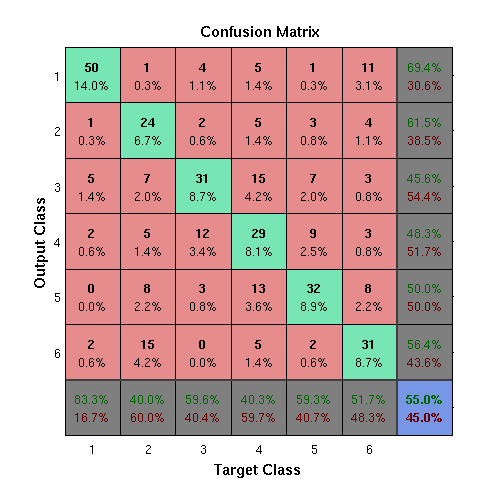
\includegraphics[width=0.5\textwidth]{figures/confusion-average}
\caption{The average confusion matrix across all subjects when the train, test, and validation sets were divided by epoch.}
\label{fig:confusion-average}
\end{figure}

\begin{figure}[!htbp]
\centering
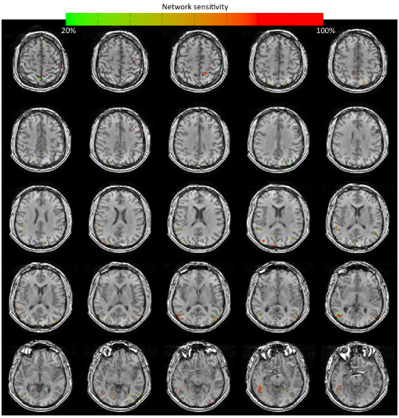
\includegraphics[width=0.5\textwidth]{figures/sensitivity-analysis}
\caption{The results of the sensitivity analysis mapped back on to the volume anatomy.}
\label{fig:sensitivity-analysis}
\end{figure}

\begin{figure}[!htbp]
\centering
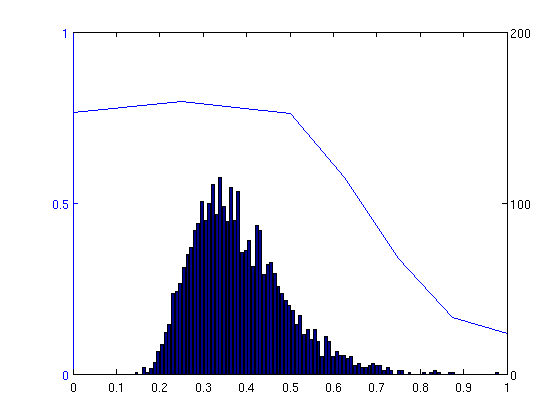
\includegraphics[width=0.5\textwidth]{figures/sensitivity-cutoff}
\caption{A histogram of the sensitivity analysis values and a plot of the feed forward neural network $F_1$ score when the inputs are pruned at a particular sensitivity value. }
\label{fig:sensitivity-cutoff}
\end{figure}

\section{Conclusions}
The reported results are well above chance, indicating there ise useflu information about character number in the BOLD signal.
The sensitivity analysis indicates that no single region of the brain is responsible for counting characters, and there is not a simple linear relationship between magnitude of activation and cardinality.
Rather, it is a complex pattern of distributed activation requiring machine-learnign methods to capture the stimulus-response relationship.

Earlier, we presnted this new trend in brain sate classification as a departure from tradiional fMRI experiments which seek to identify the purpose or function of particular brain regions.
However, it is important to note that through sensitivity analysis these machinelearning classifiers can be repurposed for just that goal.
If a region of the brain is highly important for accurately predicting the presence of a particular stimulus then it logically follows that that region must somehow be involved in the processing of that stimulus.
Furthermore, multi-voxel non-linear machine learning classifiers can potentially identify much more complex interactions between brain regions than the simple GLM.


\bibliography{bib}

\end{document}
